\documentclass[12pt,a4paper]{article}

\usepackage{amsmath,amscd,amsbsy,amssymb,latexsym,url,bm,amsthm}
\usepackage{epsfig,graphicx,subfigure}
\usepackage{enumitem,balance}
\usepackage{wrapfig}
\usepackage{mathrsfs,euscript}
\usepackage[usenames]{xcolor}
\usepackage{hyperref}
\usepackage[vlined,ruled,linesnumbered]{algorithm2e}
\hypersetup{colorlinks=true,linkcolor=black}

\newtheorem{theorem}{Theorem}
\newtheorem{lemma}[theorem]{Lemma}
\newtheorem{proposition}[theorem]{Proposition}
\newtheorem{corollary}[theorem]{Corollary}
\newtheorem{exercise}{Exercise}
\newtheorem*{solution}{Solution}
\newtheorem{definition}{Definition}
\theoremstyle{definition}

\renewcommand{\thefootnote}{\fnsymbol{footnote}}

\newcommand{\postscript}[2]
 {\setlength{\epsfxsize}{#2\hsize}
  \centerline{\epsfbox{#1}}}

\renewcommand{\baselinestretch}{1.0}

\setlength{\oddsidemargin}{-0.365in}
\setlength{\evensidemargin}{-0.365in}
\setlength{\topmargin}{-0.3in}
\setlength{\headheight}{0in}
\setlength{\headsep}{0in}
\setlength{\textheight}{10.1in}
\setlength{\textwidth}{7in}
\makeatletter \renewenvironment{proof}[1][Proof] {\par\pushQED{\qed}\normalfont\topsep6\p@\@plus6\p@\relax\trivlist\item[\hskip\labelsep\bfseries#1\@addpunct{.}]\ignorespaces}{\popQED\endtrivlist\@endpefalse} \makeatother
\makeatletter
\renewenvironment{solution}[1][Solution] {\par\pushQED{\qed}\normalfont\topsep6\p@\@plus6\p@\relax\trivlist\item[\hskip\labelsep\bfseries#1\@addpunct{.}]\ignorespaces}{\popQED\endtrivlist\@endpefalse} \makeatother

\begin{document}
\noindent

%========================================================================
\noindent\framebox[\linewidth]{\shortstack[c]{
\Large{\textbf{Lab03-GreedyStrategy}}\vspace{1mm}\\
CS214-Algorithm and Complexity, Xiaofeng Gao, Spring 2020.}}
\begin{center}
\footnotesize{\color{red}$*$ If there is any problem, please contact TA Shuodian Yu.}

% Please write down your name, student id and email.
\footnotesize{\color{blue}$*$ Name:Yulong Hui  \quad Student ID:518030910059 \quad Email: qinchuanhuiyulong@sjtu.edu.cn}
\end{center}

\begin{enumerate}
    \item
    There are $n+1$ people, each with two attributes $(a_i,b_i), i\in[0,n] \text{ and } a_i>1$. The $i$-th person can get money worth $c_i = \frac{\prod_{j=0}^{i-1}{a_j}}{b_i}$. We do not want anyone to get too much. Thus, please design a strategy to sort people from $1$ to $n$, such that the maximum earned money $c_{max}=\max\limits_{1\leq i\leq n} c_i$ is minimized. (Note: the 0-th person doesn't enroll in the sorting process, but $a_0$ always works for each $c_i$.)
    \begin{enumerate}
        \item Please design an algorithm based on greedy strategy to solve the above problem. (Write a pseudocode)
        \item Prove your algorithm is optimal.
    \end{enumerate}

  \begin{solution}
  	~\\
  	(a)The pseudocode is as follow, and  it is based on quicksort. The sequence is sorted nondecreasingly with the product of a and b.
  	  
      \begin{minipage}[t]{0.8\textwidth}
     	\begin{algorithm}[H]
     		\KwIn{An array $Person[1,\cdots,n]$}
     		\KwOut{$Person[1,\cdots,n]$ sorted nondecreasingly with $Person.a*Person.b$}
     		
     		\BlankLine
     		\caption{Sort}\label{Alg_Quick}
     		
     		\If{$n \le 1$}{
     		  \Return\;
     		}
     		
     		$pivot \leftarrow A[n]$; $i \leftarrow 1$\;
     		\For{$j \leftarrow 1$ \KwTo $n-1$}{
     			\If{$Person[j].a*Person[j].b < pivot.a*pivot.b$}{
     				swap $Person[i]$ and $Person[j]$\;
     				$i \leftarrow i+1$\;
     			}
     		}
     		
     		swap $Person[i]$ and $Person[n]$\;
     		\lIf{$i>1$}{$\operatorname{Sort}(Person[1,\cdots,i-1])$}
     		\lIf{$i<n$}{$\operatorname{Sort}(Person[i+1,\cdots,n])$}
     	\end{algorithm}
     \end{minipage}
    \end{solution}
   
   (b)
   Firstly, in a sequence, we can say there is a inversion pair. if there is a number i satsifying: $$ Person[i].a*Person[i].b > Person[i+1].a*Person[i+1].b$$
   
   If we need to prove the correctness of the greedy algorithm, we just need to prove that swappping a inversion pair will not make the final result worse.
   
   Then we just use $a_i$ and $b_i$ instead of $Person[i].a$ and $Person[i].b$.
   We suppose the oringinal case is: $a_i*b_i > a_{i+1}*b_{i+1}$, which is a inversion  pair. Obviously, the swapping will not affect other values, so we just pay attention to $c_i$ and $c_{i+1}$.
   
   Assume $c_i=\frac{A}{b_i}$, then $c_{i+1}=\frac{A*a_i}{b_{i+1}}$
   
   Because: $a_i*b_i>a_{i+1}*b_{i+1}>b_{i+1}$, we can get: $c_{i+1}$ is bigger.
   
   Then we do the swapping, and let $d_i=\frac{A}{b_{i+1}}$, then $d_{i+1}=\frac{A*a_{i+1}}{b_i}$
   
   Then, both $d_{i}$ and $d_{i+1}$ are smaller than $c_{i+1}$, because $a_i*b_i > a_{i+1}*b_{i+1}$.
   
   So, after the swapping, the maximum of the two is smaller than the old one. 
   
   Then the algorithm is proved.
   
   
   
   
 

    \item
    \textbf{Interval Scheduling} is a classic problem solved by greedy algorithm and we have introduced it in the lecture: given $n$ jobs and the $j$-th job starts at $s_j$ and finishes at $f_j$. Two jobs are compatible if they do not overlap. The goal is to find maximum subset of mutually compatible jobs. Tim wants to solve it by sort the jobs in descending order of $s_j$. Is this attempt correct? Prove the correctness of such idea, or else provide a counter-example.

   \begin{proof}
        
    
    	This idea is correct, we can prove that by contradiction.
    	
    	First we use the greedy algorithm to get a subset. Then we sort its elements (jobs) in chronological order, which will not change the number of elements but make our following analyze clearly.
    	 	
    	
    	Assume that the greedy algorithm is not the optimal algorithm, and the last $k$ jobs ($k$ is the largest possible value) in the greedy subset are the same as these in the optimal subset.(Both subset is ordered chronological)
    	\begin{figure}[h]
    		\centering
    		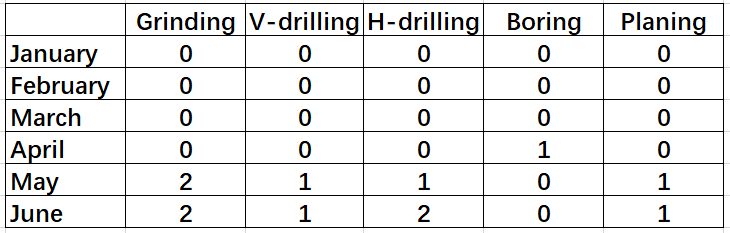
\includegraphics[width=14cm]{1.png}
    		\caption{Job Sequence}
    		
    	\end{figure}
    	
    	
    	
    	As you can see in the Figure1, the elements in job always have a bigger start time. Therefore, we can change the $k+1$ job in OPT to the $k+1$ one in Greedy sequence without affect  other earlier jobs. 
    	
    	So after the change, the  solution will still be feasible and optimal.However it contradicts the largest attribute of $k$, so the assumption is not right. The greedy algorithm is optimal. 
    	
    	
    	 
    	

        
        




  \end{proof}

    \item
    There are $n$ lectures numbered from $1$ to $n$. Lecture $i$ has duration (course length) $t_i$ and will close on $d_i$-th day. That is, you could take lecture $i$ \textbf{continuously} for $t_i$ days and must finish before or on the $d_i$-th day. The goal is to find the maximal number of courses that can be taken. (Note: you will start learning at the $1$-st day.)
    
    Please design an algorithm based on greedy strategy to solve it. You could use the data structrue learned on Data Structrue course. You need to write pseudo code and prove its correctness.

    \begin{solution}
%       Uncomment this block to write your proof.

    ~\\
     I will  explain the line-5 in the following algorithm:
     
     This "compatiable" means that : $t_j+t_{all}<d_j$ ($t_{all}$ is the total time to finish all lectures in the que).
     
    \begin{minipage}[t]{0.9\textwidth}
    	\begin{algorithm}[H]
    		\KwIn{An array $Lec[1,\cdots,n]$}
    		\KwOut{The maximal number of the lectures}
    		
    		\BlankLine
    		\caption{Greedy Schedule}\label{Alg}
    		
    		%\If{$n \le 1$}{
    		%  \Return\;
    		%}
    		
    		Sort Lectures by deadline so that 
    		$d_1<d_2<d_3<\cdots<d_n$\;
    		Create a PriorityQueue called que, which is sorted by duration($Lec[i].t$) \;
    		
    		que$\leftarrow$ $\emptyset$\;
    		
    		
    		\For{$j \leftarrow 1$ \KwTo $n$}{
    			\If{Lec[j]  \text{is compatiable with que}}{
    				Push $Lec[j]$ into the que\;
    			}
    		\Else{\If {Lec[j].t \text{is smaller than the biggest one in que}}
    		{ Pop the old biggest one out and push $Lec[j]$ in }
    	}
    		    		}
    		
    	Return the number of elements in que \;
    	\end{algorithm}
    \end{minipage}

   
    
    \begin{proof}
    	To prove the algorithm, we first need to clear two points:
    	(1) if there are two lectures with $(t_i,d_i)$ , $(t_j,d_j)$ and $d_i<d_j$
    	, then the lecture-j should be arranged after the lecture-i.
    	
    	Then,prove it:
    	
    	Let the already arranged lectures have a $t_{all}$. Then if we  arrange lecture-i after lecture-j, it must satisfy:
    	$$t_{all}+t_j\leq d_j \text{ and } t_{all}+t_j+t_i\leq d_i \eqno(1) $$
    	while another arrangement needs:
    	$$t_{all}+t_i\leq d_i \text{ and } t_{all}+t_i+t_j\leq d_j \eqno(2)$$
    	
    	Because $d_i<d_j$, if (1) is true, then (2) must be true. Otherwise it doesn't hold.
    	
    	That's to say the second arrangement can permit not less lectures.
    	
    	(2) If the next lecture is incompatible, we replace the one of biggest $t$ in the old arrangement with the new lecure of smaller $t$ (line7--line9 in algorithm). This opertion will not make the matter worse.
         
        It is because that after the exchange, the number (before the larger $d$)  will not lower, and the total time of this lectures are reduced, which will provide the later lecture with more space.
        
        Then we can prove the algorithm by induction.
        
       \textbf{Basis.}  If there is only one lecture in arrangement, the greedy one is optimal.
        
        \textbf{Assumption.}  If there have been k lectures in arrangement, the greedy one is optimal.
        
       \textbf{Induction.} Now we want to solve k+1 lectures. 
       
       Because of the point(1),  the next lecture to consider will have smallest $d$, which is optimal.
        
        If the next one is compatible with the old sequence, just add it into the consequence, then the optimal number of will be k+1 .
        
        If the next one is incompatiable then we just keep doing  the replacement (as line7--line9 in algorithm) until the compatiable one appears or the lecures are traversed. According to the point(3), it will still remain optimal.
        
        Therefore, the algorithm is proved optimal. 
        
        
    	
    	
    	
    %	So we can change the OPT into a new order, which will not lower the number of lectures.
    	
   % 	Now we compare the new ordered OPT with the Greedy. 
    	
    %	Assume that the greedy algorithm is not the optimal algorithm, and the fisrt $k$ lectures ($k$ is the largest possible value) in the greedy subset are the same as these in the optimal subset.
    %	Considering to the swap opertion (line7~line9) in algorithm, the k+1 lecture in Greedy has a smaller $t_{g}$ but a larger $d_{g}$ than that $t_{opt},d_{opt}$ in OPT. 
    	
    %	Becuse of the incompatibility, if we extend the time in OPT from $d_{}  
    	
    	
    	
    	
    	 
    \end{proof}
    

    \end{solution}

    \item
    Let $S_1,S_2,\dots,S_n$ be a partition of $S$ and $k_1,k_2,\dots,k_n$ be positive integers. Let $\mathcal{I}=\{I: I \subseteq S,|I \cap S_i| \leq k_i \text { for all } 1 \leq i \leq n\}$. Prove that $\mathcal{M}=(S,\mathcal{I})$ is a matroid.

   \begin{proof}
   ~\\
   $\bullet$ \textbf{Hereditary} Assume  $I_n \in \mathcal{I}$ and $ I_m \subseteq I_n$.
   
    Then $|I_n \cap S_i| \leq k_i \text { for all } 1 \leq i \leq n$, and $I_m$ just has some of elements in $I_n   $.
   
   
   Therefore, $|I_m \cap S_i| \leq k_i \text { for all } 1 \leq i \leq n$, which means  $I_m \in \mathcal{I}$. 
   
   Then $(S,\mathcal{I})$ is an independent system.
   
    $\bullet$ \textbf{Exchange Property}
    
    Consider $A,B\in \mathcal{I}$, and $|A|<|B|$. Then there must be a partiton of $A,B$: $$A_1,A_2,\cdots,A_n\; (A_j=A\cap S_j)$$
    $$B_1,B_2,\cdots,B_n\; (B_j=B\cap S_j)$$
    
    Because $|A|<|B|$, which means $|A_1|+\cdots+|A_n|<|B_1|+\cdots+|B_n|$, there must exists a number $i$ satisfying $|A_i|<|B_i|\leq k_i$.
    
    Then we choose $x \in B_i\backslash A_i$, and $|A_i\cup {x}|=|A_i|+1\leq k_i$.
    
    Since other part don't have any change, $A \cup {x} \in \mathcal{I}$. And the matroid is proved.  
    
     
   
    \end{proof}

\end{enumerate}

\vspace{20pt}

\textbf{Remark:} You need to include your .pdf and .tex files in your uploaded .rar or .zip file.

%========================================================================
\end{document}
